\documentclass{article}
\usepackage[paperwidth=86cm,paperheight=56cm,margin=0.8cm]{geometry}
\usepackage{fontspec}
\usepackage{amsmath}
\usepackage{unicode-math}
\setmainfont{texgyreheros}[Extension=.otf,UprightFont=*-regular,BoldFont=*-bold,ItalicFont=*-italic,BoldItalicFont=*-bolditalic]
\setmathfont{texgyrepagella-math.otf}
\usepackage[table]{xcolor}
\usepackage{tikz}
\usetikzlibrary{arrows.meta,positioning,calc,backgrounds}
\usepackage{adjustbox}
\pagestyle{empty}

\definecolor{ink}{HTML}{14213D}
\definecolor{trust}{HTML}{2F7A4F}
\definecolor{curious}{HTML}{C8611E}
\definecolor{untrusted}{HTML}{A23B3B}
\definecolor{chan}{HTML}{2F5F98}
\definecolor{soft}{HTML}{F3EFE6}
\definecolor{softblue}{HTML}{E6EEF8}
\definecolor{softgreen}{HTML}{E4F1E8}
\definecolor{softred}{HTML}{F6E3E1}
\definecolor{grey}{HTML}{6B7280}
\definecolor{bankc}{HTML}{1F6F8B}
\definecolor{keyc}{HTML}{8E2C6E}
\definecolor{gold}{HTML}{9A6B00}
\definecolor{softgold}{HTML}{FBF3DC}

\newcommand{\bk}{\tikz[baseline=(c.base)]\node[fill=bankc,text=white,rounded corners=1pt,inner sep=1.4pt,font=\bfseries\fontsize{7}{7}\selectfont] (c) {bank};}
\newcommand{\ek}{\tikz[baseline=(c.base)]\node[fill=keyc,text=white,rounded corners=1pt,inner sep=1.4pt,font=\bfseries\fontsize{7}{7}\selectfont] (c) {enclave};}
\newcommand{\pp}[1]{\tikz[baseline=(c.base)]\node[draw=ink,text=ink,rounded corners=1pt,inner sep=1.2pt,font=\bfseries\fontsize{7}{7}\selectfont] (c) {#1};}
\newcommand{\disk}[1]{\tikz[baseline=(c.base)]\node[fill=grey!20,draw=grey,text=ink,rounded corners=1pt,inner sep=1.4pt,font=\ttfamily\fontsize{7.6}{7.6}\selectfont] (c) {\detokenize{#1}};}
\newcommand{\kk}[1]{\tikz[baseline=(c.base)]\node[fill=softgold,draw=gold,text=gold,rounded corners=1pt,inner sep=1.4pt,font=\bfseries\fontsize{7.4}{7.4}\selectfont] (c) {#1};}
\newcommand{\num}[1]{\tikz[baseline=(c.base)]\node[circle,fill=ink,text=white,inner sep=1pt,font=\bfseries\fontsize{7.6}{7.6}\selectfont] (c) {#1};}
\newcommand{\cd}[1]{{\ttfamily\detokenize{#1}}}
\newcommand{\hd}[1]{{\bfseries #1}}
\newcommand{\sm}{\fontsize{9.8}{11.8}\selectfont}
\newcommand{\xs}{\fontsize{8.8}{10.6}\selectfont}

\tikzset{
  lane/.style={draw=grey!60,dashed,line width=0.6pt},
  head/.style={draw,rounded corners=3pt,line width=1.1pt,font=\sm\bfseries,minimum width=6.4cm,minimum height=1.3cm,align=center},
  note/.style={draw=grey,fill=white,rounded corners=2pt,align=left,inner sep=4pt,font=\xs},
  file/.style={draw=grey,fill=grey!8,align=left,inner sep=4pt,font=\xs,double,double distance=1pt},
  arr/.style={-{Stealth[length=7pt]},line width=1pt,ink},
  sarr/.style={-{Stealth[length=7pt]},line width=1pt,chan},
  darr/.style={-{Stealth[length=7pt]},line width=0.9pt,grey,dashed},
  msg/.style={font=\xs,fill=white,inner sep=1.5pt,align=center},
  phase/.style={font=\sm\bfseries,text=grey,anchor=south west,inner sep=2pt},
}

\newcommand{\call}[6][arr]{%
  \node[msg,anchor=north,text width=#4] (#6l) at ($(cur -| #2)!0.5!(cur -| #3)$) {#5};
  \coordinate (#6) at ($(#6l.south)+(0,-0.14)$);
  \draw[#1] (#6 -| #2) -- (#6 -| #3);
  \coordinate (cur) at ($(#6)+(0,-0.4)$);
}
\newcommand{\after}[2][0.35]{\coordinate (cur) at ($(#2.south)+(0,-#1)$);}
\newcommand{\aftertwo}[3][0.35]{\path let \p1=(#2.south), \p2=(#3.south) in coordinate (cur) at (0,{min(\y1,\y2)-#1 cm});}
\newcommand{\phaseline}[1]{%
  \coordinate (cur) at ($(cur)+(0,-0.55)$);
  \draw[grey!45,line width=0.8pt] ($(cur -| L0)+(0,-0.1)$) -- ($(cur -| L9)+(0,-0.1)$);
  \node[phase] at ($(cur -| L0)+(0,-0.05)$) {#1};
  \coordinate (cur) at ($(cur)+(0,-0.75)$);
}

\begin{document}
\hyphenpenalty=10000\exhyphenpenalty=10000
\noindent
\begin{adjustbox}{max width=\linewidth,max totalheight=0.98\textheight,center}
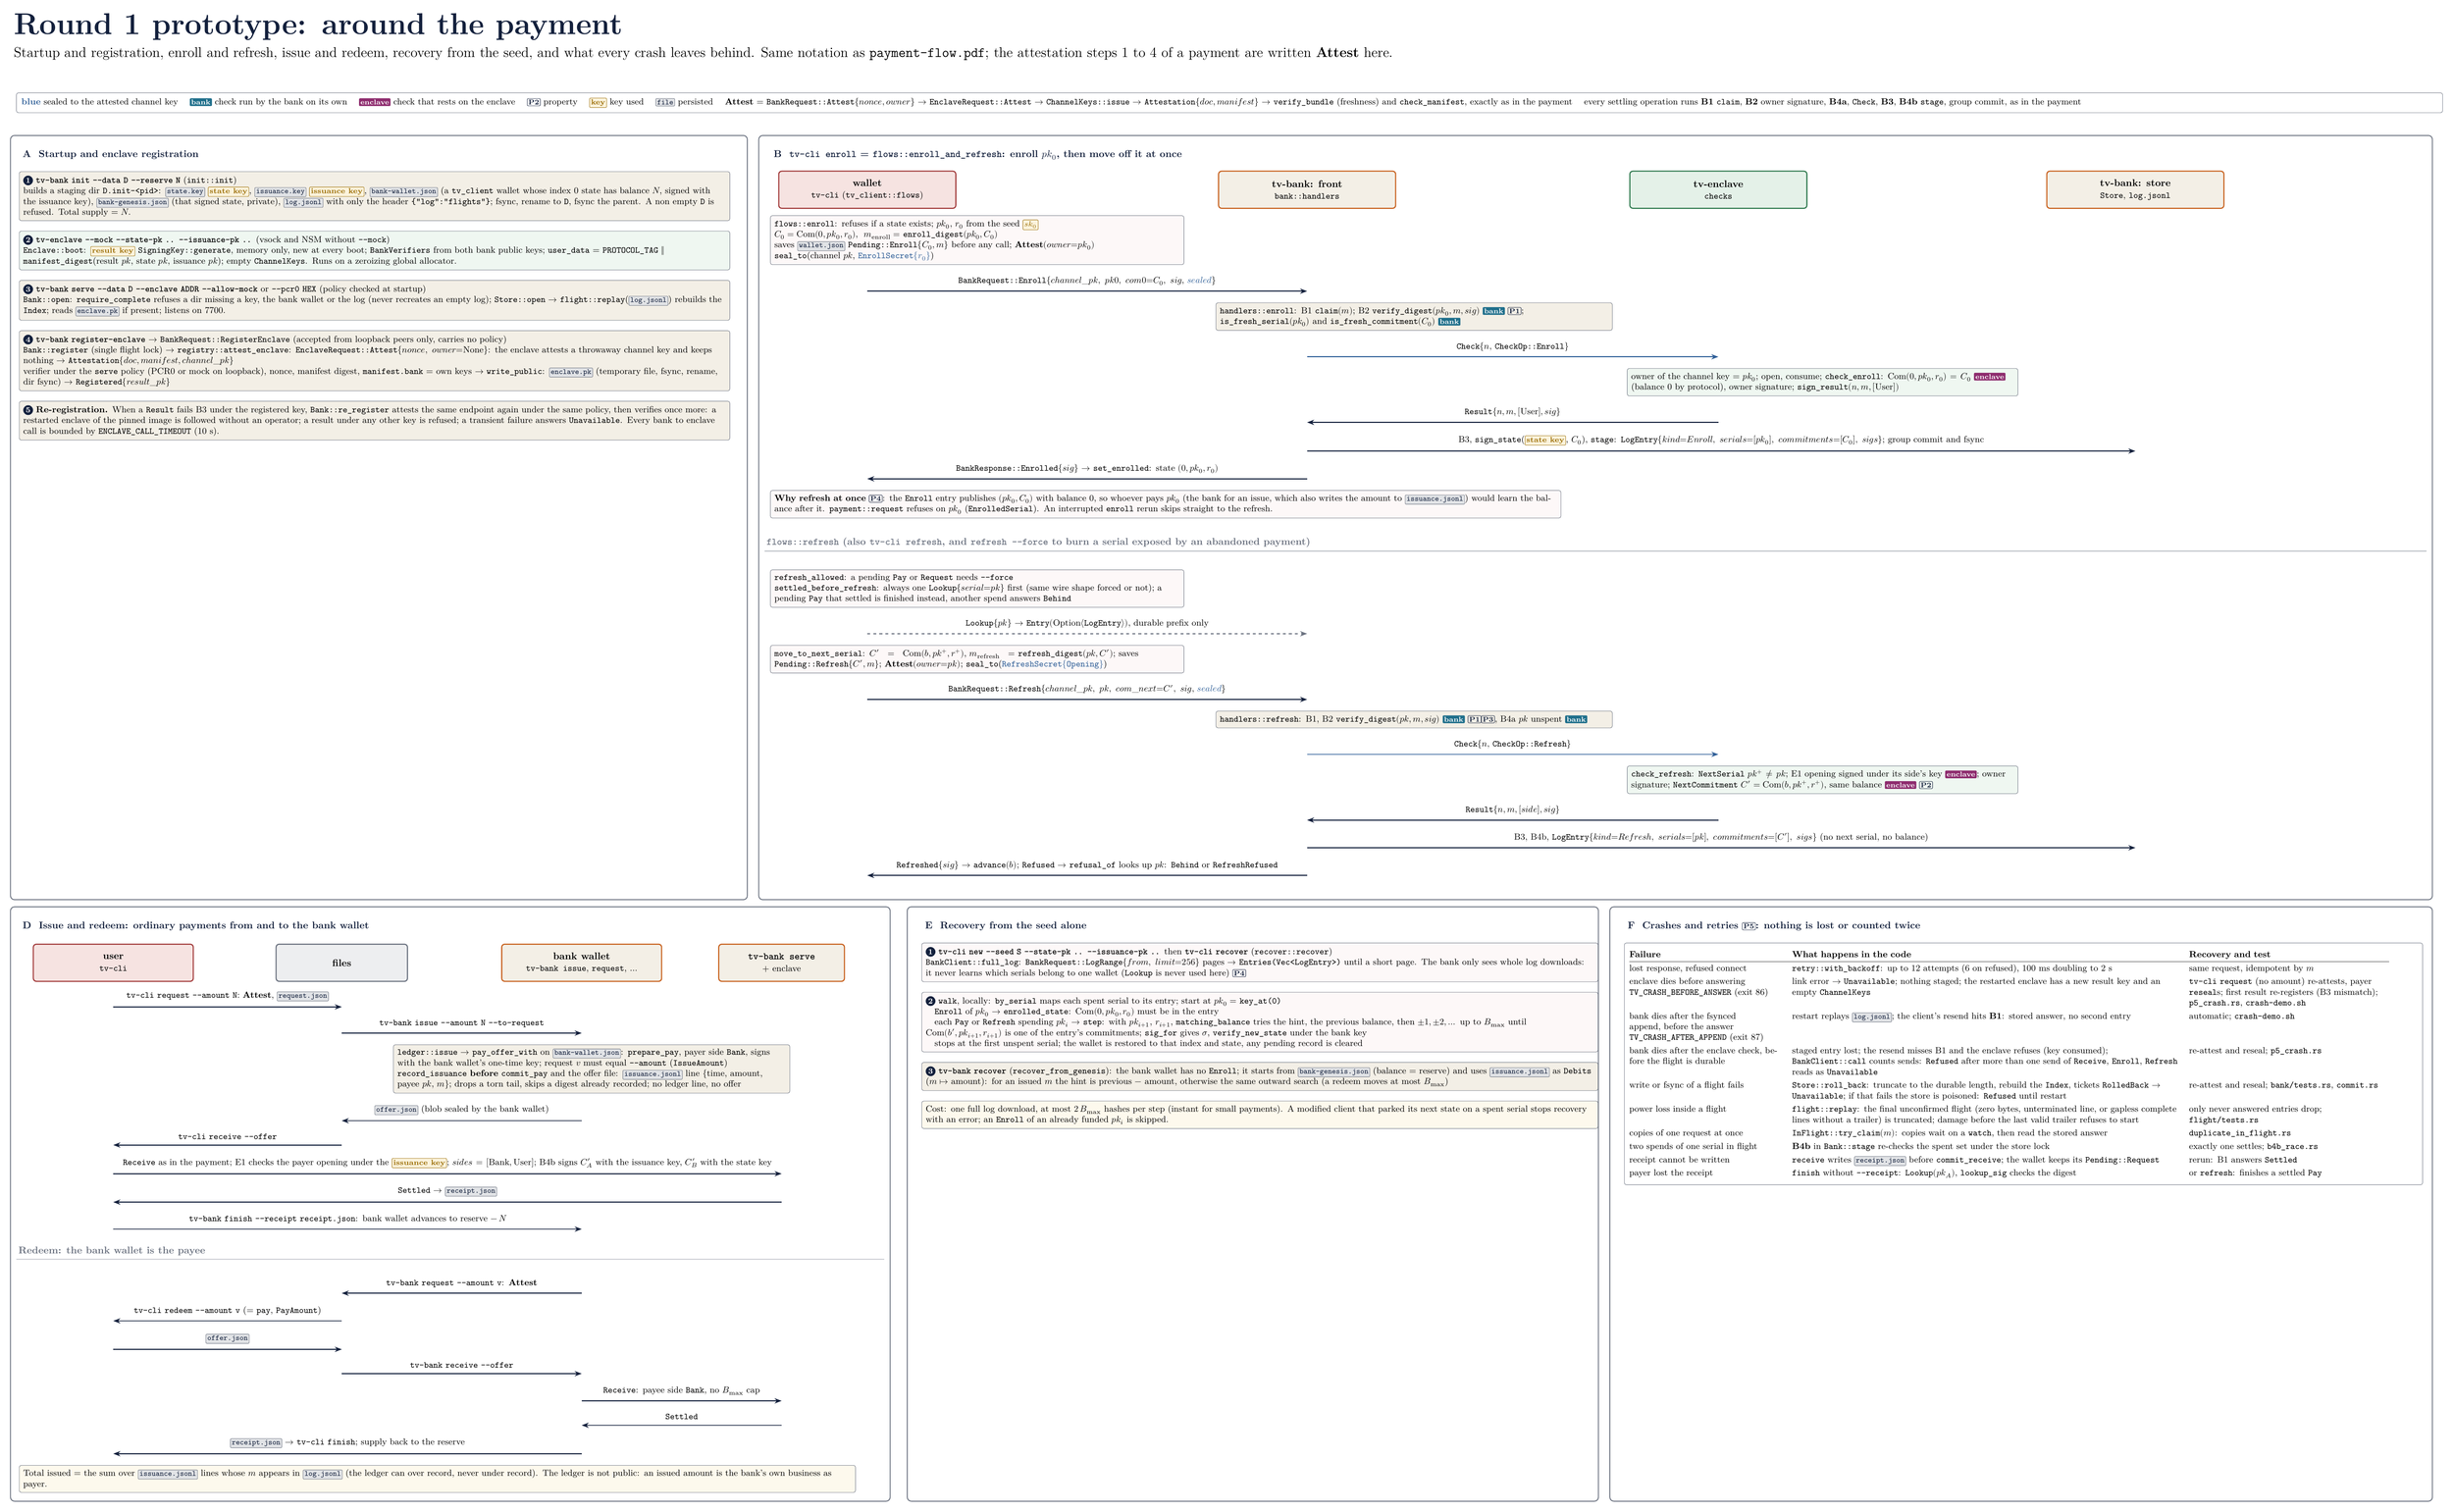
\begin{tikzpicture}[x=1cm,y=1cm]

\node[anchor=north west,align=left] at (0,58.2) {{\bfseries\fontsize{30}{34}\selectfont\color{ink} Round 1 prototype: around the payment}\\[6pt]{\fontsize{14}{17}\selectfont Startup and registration, enroll and refresh, issue and redeem, recovery from the seed, and what every crash leaves behind. Same notation as \cd{payment-flow.pdf}; the attestation steps 1 to 4 of a payment are written \hd{Attest} here.}};

\node[anchor=north west,align=left,font=\xs,draw=grey,rounded corners=2pt,inner sep=5pt,text width=84.6cm] at (0.2,55.3) {
{\color{chan}\textbf{blue}} sealed to the attested channel key \quad \bk{} check run by the bank on its own \quad \ek{} check that rests on the enclave \quad \pp{P2} property \quad \kk{key} key used \quad \disk{file} persisted \quad \hd{Attest} = \cd{BankRequest::Attest}$\{nonce, owner\}$ $\to$ \cd{EnclaveRequest::Attest} $\to$ \cd{ChannelKeys::issue} $\to$ \cd{Attestation}$\{doc, manifest\}$ $\to$ \cd{verify_bundle} (freshness) and \cd{check_manifest}, exactly as in the payment \quad every settling operation runs \hd{B1} \cd{claim}, \hd{B2} owner signature, \hd{B4a}, \cd{Check}, \hd{B3}, \hd{B4b} \cd{stage}, group commit, as in the payment};

\coordinate (pAtop) at (0,53.6);
\node[anchor=north west,font=\sm\bfseries,text=ink] (tA) at ($(pAtop)+(0.3,-0.2)$) {A \ Startup and enclave registration};
\node[note,anchor=north west,text width=24.6cm,fill=soft] (a1) at ($(tA.south west)+(0,-0.3)$) {\num{1} \hd{\cd{tv-bank init --data D --reserve N}} (\cd{init::init})\\
builds a staging dir \cd{D.init-<pid>}: \disk{state.key} \kk{state key}, \disk{issuance.key} \kk{issuance key}, \disk{bank-wallet.json} (a \cd{tv_client} wallet whose index 0 state has balance $N$, signed with the issuance key), \disk{bank-genesis.json} (that signed state, private), \disk{log.jsonl} with only the header \cd{{"log":"flights"}}; fsync, rename to \cd{D}, fsync the parent. A non empty \cd{D} is refused. Total supply = $N$.};
\node[note,anchor=north west,text width=24.6cm,fill=softgreen!60] (a2) at ($(a1.south west)+(0,-0.35)$) {\num{2} \hd{\cd{tv-enclave --mock --state-pk .. --issuance-pk ..}} (vsock and NSM without \cd{--mock})\\
\cd{Enclave::boot}: \kk{result key} \cd{SigningKey::generate}, memory only, new at every boot; \cd{BankVerifiers} from both bank public keys; \cd{user_data} = \cd{PROTOCOL_TAG} $\|$ \cd{manifest_digest}(result $pk$, state $pk$, issuance $pk$); empty \cd{ChannelKeys}. Runs on a zeroizing global allocator.};
\node[note,anchor=north west,text width=24.6cm,fill=soft] (a3) at ($(a2.south west)+(0,-0.35)$) {\num{3} \hd{\cd{tv-bank serve --data D --enclave ADDR --allow-mock}} or \cd{--pcr0 HEX} (policy checked at startup)\\
\cd{Bank::open}: \cd{require_complete} refuses a dir missing a key, the bank wallet or the log (never recreates an empty log); \cd{Store::open} $\to$ \cd{flight::replay}(\disk{log.jsonl}) rebuilds the \cd{Index}; reads \disk{enclave.pk} if present; listens on 7700.};
\node[note,anchor=north west,text width=24.6cm,fill=soft] (a4) at ($(a3.south west)+(0,-0.35)$) {\num{4} \hd{\cd{tv-bank register-enclave}} $\to$ \cd{BankRequest::RegisterEnclave} (accepted from loopback peers only, carries no policy)\\
\cd{Bank::register} (single flight lock) $\to$ \cd{registry::attest_enclave}: \cd{EnclaveRequest::Attest}$\{nonce,\ owner{=}\mathrm{None}\}$: the enclave attests a throwaway channel key and keeps nothing $\to$ \cd{Attestation}$\{doc, manifest, channel\_pk\}$\\
verifier under the \cd{serve} policy (PCR0 or mock on loopback), nonce, manifest digest, \cd{manifest.bank} = own keys $\to$ \cd{write_public}: \disk{enclave.pk} (temporary file, fsync, rename, dir fsync) $\to$ \cd{Registered}$\{result\_pk\}$};
\node[note,anchor=north west,text width=24.6cm,fill=soft] (a5) at ($(a4.south west)+(0,-0.35)$) {\num{5} \hd{Re-registration.} When a \cd{Result} fails B3 under the registered key, \cd{Bank::re_register} attests the same endpoint again under the same policy, then verifies once more: a restarted enclave of the pinned image is followed without an operator; a result under any other key is refused; a transient failure answers \cd{Unavailable}. Every bank to enclave call is bounded by \cd{ENCLAVE_CALL_TIMEOUT} (10 s).};
\coordinate (Abot) at ($(a5.south)+(0,-0.4)$);

\def\bW{30.0}\def\bK{45.4}\def\bE{59.8}\def\bS{74.4}
\coordinate (LW) at (\bW,0);
\coordinate (LK) at (\bK,0);
\coordinate (LE) at (\bE,0);
\coordinate (LS) at (\bS,0);
\coordinate (L0) at (26.4,0);
\coordinate (L9) at (84.6,0);
\node[anchor=north west,font=\sm\bfseries,text=ink] (tB) at (26.6,53.4) {B \ \cd{tv-cli enroll} = \cd{flows::enroll_and_refresh}: enroll $pk_0$, then move off it at once};
\node[head,draw=untrusted,fill=softred,minimum width=6.2cm] at (\bW,51.9) {wallet\\{\xs\mdseries\cd{tv-cli} (\cd{tv_client::flows})}};
\node[head,draw=curious,fill=soft,minimum width=6.2cm] at (\bK,51.9) {tv-bank: front\\{\xs\mdseries\cd{bank::handlers}}};
\node[head,draw=trust,fill=softgreen,minimum width=6.2cm] at (\bE,51.9) {tv-enclave\\{\xs\mdseries\cd{checks}}};
\node[head,draw=curious,fill=soft,minimum width=6.2cm] at (\bS,51.9) {tv-bank: store\\{\xs\mdseries\cd{Store}, \cd{log.jsonl}}};
\coordinate (Btop) at (0,51.2);
\coordinate (cur) at (0,51.0);

\node[note,anchor=north west,text width=14.2cm,fill=softred!25] (be1) at ($(cur -| LW)+(-3.4,0)$) {\cd{flows::enroll}: refuses if a state exists; $pk_0$, $r_0$ from the seed \kk{$sk_0$}\\
$C_0=\mathrm{Com}(0, pk_0, r_0)$, \ $m_{\text{enroll}}=$ \cd{enroll_digest}$(pk_0, C_0)$\\
saves \disk{wallet.json} \cd{Pending::Enroll}$\{C_0, m\}$ before any call; \hd{Attest}$(owner{=}pk_0)$\\
\cd{seal_to}(channel $pk$, {\color{chan}\cd{EnrollSecret}$\{r_0\}$})};
\after{be1}
\call{LW}{LK}{14cm}{\cd{BankRequest::Enroll}$\{channel\_pk,\ pk0,\ com0{=}C_0,\ sig,$ {\color{chan}$sealed$}$\}$}{ba1}
\node[note,anchor=north west,text width=13.6cm,fill=soft] (bk1) at ($(cur -| LK)+(-3.2,0)$) {\cd{handlers::enroll}: B1 \cd{claim}$(m)$; B2 \cd{verify_digest}$(pk_0, m, sig)$ \bk{} \pp{P1}; \cd{is_fresh_serial}$(pk_0)$ and \cd{is_fresh_commitment}$(C_0)$ \bk{}};
\after{bk1}
\call[sarr]{LK}{LE}{13.6cm}{\cd{Check}$\{n,$ \cd{CheckOp::Enroll}$\}$}{ba2}
\node[note,anchor=north west,text width=13.4cm,fill=softgreen!60] (be2) at ($(cur -| LE)+(-3.2,0)$) {owner of the channel key = $pk_0$; open, consume; \cd{check_enroll}: $\mathrm{Com}(0, pk_0, r_0)=C_0$ \ek{} (balance 0 by protocol), owner signature; \cd{sign_result}$(n, m, [\text{User}])$};
\after{be2}
\call{LE}{LK}{13.6cm}{\cd{Result}$\{n, m, [\text{User}], sig\}$}{ba3}
\call{LK}{LS}{28cm}{B3, \cd{sign_state}(\kk{state key}, $C_0$), \cd{stage}: \cd{LogEntry}$\{kind{=}Enroll,\ serials{=}[pk_0],\ commitments{=}[C_0],\ sigs\}$; group commit and fsync}{ba4}
\call{LK}{LW}{14cm}{\cd{BankResponse::Enrolled}$\{sig\}$ $\to$ \cd{set_enrolled}: state $(0, pk_0, r_0)$}{ba5}
\node[note,anchor=north west,text width=27.4cm,fill=softred!25] (bw) at ($(cur -| LW)+(-3.4,0)$) {\hd{Why refresh at once} \pp{P4}: the \cd{Enroll} entry publishes $(pk_0, C_0)$ with balance 0, so whoever pays $pk_0$ (the bank for an issue, which also writes the amount to \disk{issuance.jsonl}) would learn the balance after it. \cd{payment::request} refuses on $pk_0$ (\cd{EnrolledSerial}). An interrupted \cd{enroll} rerun skips straight to the refresh.};
\after[0.5]{bw}
\phaseline{\cd{flows::refresh} (also \cd{tv-cli refresh}, and \cd{refresh --force} to burn a serial exposed by an abandoned payment)}
\node[note,anchor=north west,text width=14.2cm,fill=softred!25] (br1) at ($(cur -| LW)+(-3.4,0)$) {\cd{refresh_allowed}: a pending \cd{Pay} or \cd{Request} needs \cd{--force}\\
\cd{settled_before_refresh}: always one \cd{Lookup}$\{serial{=}pk\}$ first (same wire shape forced or not); a pending \cd{Pay} that settled is finished instead, another spend answers \cd{Behind}};
\after{br1}
\call[darr]{LW}{LK}{14cm}{\cd{Lookup}$\{pk\}$ $\to$ \cd{Entry}$(\mathrm{Option}\langle$\cd{LogEntry}$\rangle)$, durable prefix only}{bb0}
\node[note,anchor=north west,text width=14.2cm,fill=softred!25] (br2) at ($(cur -| LW)+(-3.4,0)$) {\cd{move_to_next_serial}: $C'=\mathrm{Com}(b, pk^{+}, r^{+})$, $m_{\text{refresh}}=$ \cd{refresh_digest}$(pk, C')$; saves \cd{Pending::Refresh}$\{C', m\}$; \hd{Attest}$(owner{=}pk)$; \cd{seal_to}({\color{chan}\cd{RefreshSecret}$\{$\cd{Opening}$\}$})};
\after{br2}
\call{LW}{LK}{14cm}{\cd{BankRequest::Refresh}$\{channel\_pk,\ pk,\ com\_next{=}C',\ sig,$ {\color{chan}$sealed$}$\}$}{bb1}
\node[note,anchor=north west,text width=13.6cm,fill=soft] (bk2) at ($(cur -| LK)+(-3.2,0)$) {\cd{handlers::refresh}: B1, B2 \cd{verify_digest}$(pk, m, sig)$ \bk{} \pp{P1}\pp{P3}, B4a $pk$ unspent \bk{}};
\after{bk2}
\call[sarr]{LK}{LE}{13.6cm}{\cd{Check}$\{n,$ \cd{CheckOp::Refresh}$\}$}{bb2}
\node[note,anchor=north west,text width=13.4cm,fill=softgreen!60] (be3) at ($(cur -| LE)+(-3.2,0)$) {\cd{check_refresh}: \cd{NextSerial} $pk^{+}\ne pk$; E1 opening signed under its side's key \ek{}; owner signature; \cd{NextCommitment} $C'=\mathrm{Com}(b, pk^{+}, r^{+})$, same balance \ek{} \pp{P2}};
\after{be3}
\call{LE}{LK}{13.6cm}{\cd{Result}$\{n, m, [side], sig\}$}{bb3}
\call{LK}{LS}{28cm}{B3, B4b, \cd{LogEntry}$\{kind{=}Refresh,\ serials{=}[pk],\ commitments{=}[C'],\ sigs\}$ (no next serial, no balance)}{bb4}
\call{LK}{LW}{14cm}{\cd{Refreshed}$\{sig\}$ $\to$ \cd{advance}$(b)$; \cd{Refused} $\to$ \cd{refusal_of} looks up $pk$: \cd{Behind} or \cd{RefreshRefused}}{bb5}
\coordinate (Bbot) at (cur);
\begin{scope}[on background layer]
\foreach \l in {LW,LK,LE,LS} {\draw[lane] (Btop -| \l) -- (Bbot -| \l);}
\end{scope}

\path let \p1=(Abot), \p2=(Bbot) in coordinate (row2) at (0,{min(\y1,\y2)-0.9cm});
\begin{scope}[on background layer]
\draw[grey,rounded corners=4pt,line width=0.9pt,fill=white] ($(pAtop)+(0,0.2)$) rectangle ($(row2)+(25.8,0.45)$);
\draw[grey,rounded corners=4pt,line width=0.9pt,fill=white] ($(pAtop)+(26.2,0.2)$) rectangle ($(row2)+(84.8,0.45)$);
\end{scope}

\def\dU{3.6}\def\dF{11.6}\def\dW{20.0}\def\dK{27.0}
\coordinate (LU) at (\dU,0);
\coordinate (LF) at (\dF,0);
\coordinate (LW) at (\dW,0);
\coordinate (LK) at (\dK,0);
\coordinate (L0) at (0.2,0);
\coordinate (L9) at (30.6,0);
\node[anchor=north west,font=\sm\bfseries,text=ink] (tD) at ($(row2)+(0.3,-0.2)$) {D \ Issue and redeem: ordinary payments from and to the bank wallet};
\path let \p1=(tD.south) in coordinate (Dhead) at (0,\y1-1.0cm);
\node[head,draw=untrusted,fill=softred,minimum width=5.6cm] at (Dhead -| LU) {user\\{\xs\mdseries\cd{tv-cli}}};
\node[head,draw=grey,fill=grey!12,minimum width=4.6cm] at (Dhead -| LF) {files};
\node[head,draw=curious,fill=soft,minimum width=5.6cm] at (Dhead -| LW) {bank wallet\\{\xs\mdseries\cd{tv-bank issue}, \cd{request}, ...}};
\node[head,draw=curious,fill=soft,minimum width=4.4cm] at (Dhead -| LK) {\cd{tv-bank serve}\\{\xs\mdseries + enclave}};
\coordinate (Dtop) at ($(Dhead)+(0,-0.7)$);
\coordinate (cur) at ($(Dhead)+(0,-0.95)$);
\call{LU}{LF}{7.6cm}{\cd{tv-cli request --amount N}: \hd{Attest}, \disk{request.json}}{d1}
\call{LF}{LW}{7.6cm}{\cd{tv-bank issue --amount N --to-request}}{d2}
\node[note,anchor=north west,text width=13.6cm,fill=soft] (dn1) at ($(cur -| LW)+(-6.6,0)$) {\cd{ledger::issue} $\to$ \cd{pay_offer_with} on \disk{bank-wallet.json}: \cd{prepare_pay}, payer side \cd{Bank}, signs with the bank wallet's one-time key; request $v$ must equal \cd{--amount} (\cd{IssueAmount})\\
\cd{record_issuance} \hd{before} \cd{commit_pay} and the offer file: \disk{issuance.jsonl} line $\{$time, amount, payee $pk$, $m\}$; drops a torn tail, skips a digest already recorded; no ledger line, no offer};
\after{dn1}
\call{LW}{LF}{7.6cm}{\disk{offer.json} (blob sealed by the bank wallet)}{d3}
\call{LF}{LU}{7.6cm}{\cd{tv-cli receive --offer}}{d4}
\call{LU}{LK}{23.2cm}{\cd{Receive} as in the payment; E1 checks the payer opening under the \kk{issuance key}; $sides=[\text{Bank}, \text{User}]$; B4b signs $C_A'$ with the issuance key, $C_B'$ with the state key}{d5}
\call{LK}{LU}{22cm}{\cd{Settled} $\to$ \disk{receipt.json}}{d6}
\call{LU}{LW}{14cm}{\cd{tv-bank finish --receipt receipt.json}: bank wallet advances to reserve $-\,N$}{d7}
\phaseline{Redeem: the bank wallet is the payee}
\call{LW}{LF}{7.6cm}{\cd{tv-bank request --amount v}: \hd{Attest}}{d8}
\call{LF}{LU}{7.6cm}{\cd{tv-cli redeem --amount v} (= \cd{pay}, \cd{PayAmount})}{d9}
\call{LU}{LF}{7.6cm}{\disk{offer.json}}{d10}
\call{LF}{LW}{7.6cm}{\cd{tv-bank receive --offer}}{d11}
\call{LW}{LK}{6.6cm}{\cd{Receive}: payee side \cd{Bank}, no $B_{\max}$ cap}{d12}
\call{LK}{LW}{6.6cm}{\cd{Settled}}{d13}
\call{LW}{LU}{14cm}{\disk{receipt.json} $\to$ \cd{tv-cli finish}; supply back to the reserve}{d14}
\node[note,anchor=north west,text width=29cm,fill=softgold!50] (dn2) at ($(cur -| L0)+(0.1,0)$) {Total issued = the sum over \disk{issuance.jsonl} lines whose $m$ appears in \disk{log.jsonl} (the ledger can over record, never under record). The ledger is not public: an issued amount is the bank's own business as payer.};
\coordinate (Dbot) at ($(dn2.south)+(0,-0.3)$);
\begin{scope}[on background layer]
\foreach \l in {LU,LF,LW,LK} {\draw[lane] (Dtop -| \l) -- (dn2.north -| \l);}
\end{scope}

\coordinate (Ex) at (31.6,0);
\node[anchor=north west,font=\sm\bfseries,text=ink] (tE) at ($(row2 -| Ex)+(0.3,-0.2)$) {E \ Recovery from the seed alone};
\node[note,anchor=north west,text width=23.4cm,fill=softred!25] (e1) at ($(tE.south west)+(0,-0.3)$) {\num{1} \hd{\cd{tv-cli new --seed S --state-pk .. --issuance-pk ..}} then \hd{\cd{tv-cli recover}} (\cd{recover::recover})\\
\cd{BankClient::full_log}: \cd{BankRequest::LogRange}$\{from,\ limit{=}256\}$ pages $\to$ \cd{Entries(Vec<LogEntry>)} until a short page. The bank only sees whole log downloads: it never learns which serials belong to one wallet (\cd{Lookup} is never used here) \pp{P4}};
\node[note,anchor=north west,text width=23.4cm,fill=softred!25] (e2) at ($(e1.south west)+(0,-0.35)$) {\num{2} \cd{walk}, locally: \cd{by_serial} maps each spent serial to its entry; start at $pk_0=$ \cd{key_at(0)}\\
\quad \cd{Enroll} of $pk_0$ $\to$ \cd{enrolled_state}: $\mathrm{Com}(0, pk_0, r_0)$ must be in the entry\\
\quad each \cd{Pay} or \cd{Refresh} spending $pk_i$ $\to$ \cd{step}: with $pk_{i+1}$, $r_{i+1}$, \cd{matching_balance} tries the hint, the previous balance, then $\pm1, \pm2, \dots$ up to $B_{\max}$ until $\mathrm{Com}(b', pk_{i+1}, r_{i+1})$ is one of the entry's commitments; \cd{sig_for} gives $\sigma$, \cd{verify_new_state} under the bank key\\
\quad stops at the first unspent serial; the wallet is restored to that index and state, any pending record is cleared};
\node[note,anchor=north west,text width=23.4cm,fill=soft] (e3) at ($(e2.south west)+(0,-0.35)$) {\num{3} \hd{\cd{tv-bank recover}} (\cd{recover_from_genesis}): the bank wallet has no \cd{Enroll}; it starts from \disk{bank-genesis.json} (balance = reserve) and uses \disk{issuance.jsonl} as \cd{Debits} ($m \mapsto$ amount): for an issued $m$ the hint is previous $-$ amount, otherwise the same outward search (a redeem moves at most $B_{\max}$)};
\node[note,anchor=north west,text width=23.4cm,fill=softgold!50] (e4) at ($(e3.south west)+(0,-0.35)$) {Cost: one full log download, at most $2\,B_{\max}$ hashes per step (instant for small payments). A modified client that parked its next state on a spent serial stops recovery with an error; an \cd{Enroll} of an already funded $pk_i$ is skipped.};
\coordinate (Ebot) at ($(e4.south)+(0,-0.3)$);

\coordinate (Fx) at (56.2,0);
\node[anchor=north west,font=\sm\bfseries,text=ink] (tF) at ($(row2 -| Fx)+(0.3,-0.2)$) {F \ Crashes and retries \pp{P5}: nothing is lost or counted twice};
\node[note,anchor=north west,text width=27.6cm,inner sep=5pt] (f1) at ($(tF.south west)+(0,-0.3)$) {\renewcommand{\arraystretch}{1.25}%
\begin{tabular}{@{}p{5.4cm}@{\hspace{0.3cm}}p{13.6cm}@{\hspace{0.3cm}}p{7.0cm}@{}}
\hd{Failure} & \hd{What happens in the code} & \hd{Recovery and test}\\\hline
lost response, refused connect & \cd{retry::with_backoff}: up to 12 attempts (6 on refused), 100 ms doubling to 2 s & same request, idempotent by $m$\\
enclave dies before answering \cd{TV_CRASH_BEFORE_ANSWER} (exit 86) & link error $\to$ \cd{Unavailable}; nothing staged; the restarted enclave has a new result key and an empty \cd{ChannelKeys} & \cd{tv-cli request} (no amount) re-attests, payer \cd{reseal}s; first result re-registers (B3 mismatch); \cd{p5_crash.rs}, \cd{crash-demo.sh}\\
bank dies after the fsynced append, before the answer \cd{TV_CRASH_AFTER_APPEND} (exit 87) & restart replays \disk{log.jsonl}; the client's resend hits \hd{B1}: stored answer, no second entry & automatic; \cd{crash-demo.sh}\\
bank dies after the enclave check, before the flight is durable & staged entry lost; the resend misses B1 and the enclave refuses (key consumed); \cd{BankClient::call} counts sends: \cd{Refused} after more than one send of \cd{Receive}, \cd{Enroll}, \cd{Refresh} reads as \cd{Unavailable} & re-attest and reseal; \cd{p5_crash.rs}\\
write or fsync of a flight fails & \cd{Store::roll_back}: truncate to the durable length, rebuild the \cd{Index}, tickets \cd{RolledBack} $\to$ \cd{Unavailable}; if that fails the store is poisoned: \cd{Refused} until restart & re-attest and reseal; \cd{bank/tests.rs}, \cd{commit.rs}\\
power loss inside a flight & \cd{flight::replay}: the final unconfirmed flight (zero bytes, unterminated line, or gapless complete lines without a trailer) is truncated; damage before the last valid trailer refuses to start & only never answered entries drop; \cd{flight/tests.rs}\\
copies of one request at once & \cd{InFlight::try_claim}$(m)$: copies wait on a \cd{watch}, then read the stored answer & \cd{duplicate_in_flight.rs}\\
two spends of one serial in flight & \hd{B4b} in \cd{Bank::stage} re-checks the spent set under the store lock & exactly one settles; \cd{b4b_race.rs}\\
receipt cannot be written & \cd{receive} writes \disk{receipt.json} before \cd{commit_receive}; the wallet keeps its \cd{Pending::Request} & rerun: B1 answers \cd{Settled}\\
payer lost the receipt & \cd{finish} without \cd{--receipt}: \cd{Lookup}$(pk_A)$, \cd{lookup_sig} checks the digest & or \cd{refresh}: finishes a settled \cd{Pay}\\
\end{tabular}};
\coordinate (Fbot) at ($(f1.south)+(0,-0.3)$);

\path let \p1=(Dbot), \p2=(Ebot), \p3=(Fbot) in coordinate (row2b) at (0,{min(\y1,min(\y2,\y3))});
\begin{scope}[on background layer]
\draw[grey,rounded corners=4pt,line width=0.9pt,fill=white] ($(row2)+(0,0.2)$) rectangle ($(row2b)+(30.8,0)$);
\draw[grey,rounded corners=4pt,line width=0.9pt,fill=white] ($(row2)+(31.4,0.2)$) rectangle ($(row2b)+(55.6,0)$);
\draw[grey,rounded corners=4pt,line width=0.9pt,fill=white] ($(row2)+(56.0,0.2)$) rectangle ($(row2b)+(84.8,0)$);
\end{scope}

\end{tikzpicture}
\end{adjustbox}
\end{document}

